
\section{Methodology}

As discussed, the market type for the artificial market built in this thesis was chosen 
to be a continuous double auction. More specifically, the microstructure is formed as a 
limit order book market or an order-driven market with continuous clearing. The rationale 
for these decisions was that actual stock markets are often organized as such and that 
order-driven markets are more transparent than quote-driven thus they can be modelled more 
accurately. The model was written in Julia
programming language and it took inspiration from previous ASM literature.
The literature is lacking in practical studies about how to actually create
an artificial stock market and therefore to contribute to the literature %TODO Supervisor: This is important and should be highlighted in research questions: "therefore to contribute to the literature the actual structure of the market is explained in depth"
the actual structure of the market is explained in depth. The decisions 
about the microstructure and the trader behaviour most closely resembles the 
work of \citet{Genoa01} and \citet{Raberto05} whereas for the structure and 
practical implementation the inspiration was taken from the work of \citet{Ben12}. 
The goal was to create a generic artificial market model with an emphasis on flexibility 
and practicality. However, many of the features of the model are not tested in this thesis 
due to the scope of the thesis. The plotting and the analysis of the results were 
conducted using Python and its scientific computing stack including Numpy, Pandas, 
Statsmodels, Matplotlib, Seaborn and Scipy libraries. In this section the rationale 
for the programming choice of the model is discussed and the model structure, 
mechanics and generic characteristics are explained.

\subsection{Julia Language}
Julia is a relatively new dynamic programming language, 
reaching a stable release of 1.0 in August 2018 \citep{JuliaV1}.
It is a performant language with an emphasis
on productivity. Even though Julia has a focus on scientific 
computing it is considered as a general-purpose programming
language. Some of its features include
multiple dispatch, just-in-time compilation and built-in
matrix data types \citep{Julia}.

Julia fits well in building an artificial market.
Artificial markets can be seen as sets of objects
and interactions in between, as described \citet{Ben12},
and in such models object-oriented programming (OOP)
may be preferable. Even though Julia is more functional in nature, 
many of the features of OOP could be constructed with Julia's mutable structs 
and type annotated functions. Also, the speed of code execution, 
support for matrix operations and good productivity makes 
it a viable language for prototyping simulation systems. 


\subsection{Generic Structure of the Model}
% Describe the generic structure (Type hierarchy, layers etc.)
% Kind of the static side of the simulation, the abstraction dimension
The ASM model has three layers: abstraction layer, concrete 
layer and simulation layer. The first layer, abstraction layer, contains the 
generic parts of the framework that are independent and obvious in terms
of functionality. For example, how to get traders' positions, how to
transfer assets from a trader to another or how to cancel an order are
functionalities that are independent on the type of trader 
and type of markets, and therefore these functionalities have little
far-reaching decisions to make. The main purpose of this layer
is to separate generic and obvious functionality from blocks of code
that have more degrees of freedom and less obvious and harder to validate 
design decisions to make.

The second layer, the concrete layer, defines the actual types and the
functionalities that require less clear and more heuristic
approach than the abstract layer. This layer also includes a significant
portion of choices to make. Some of the components
on this layer include the zero-intelligent trader and the
functions that define its behaviour, the continuous double auction
market and the functions for its price formation mechanics.

The third layer, the simulation layer, manages the simulation as a whole.
This layer defines the ecosystem where the simulation takes place including
the initiation of the components, iterating over the time periods, asking
each trader to make their decisions and ask the market to clear. 
Also, initial conditions including the number of sessions, investors, assets and markets
and the amount of each asset each investor initially owns are defined here. 
This layer mostly calls the functionalities created in the lower layers.

The layers and components of the model are illustrated in figure ~\ref{fig:asm_structure}.
The components of the model resemble the simplified agent model of \citet{Ben12}: the model consists of 
two core components and these are the markets and the trading agents. In addition to these components, 
some additional components, such as orders, trades and assets, were also implemented to maintain readability 
in the code and to provide flexibility. Some of the functionalities 
of the service model they designed were also implemented including \textit{generating orders}, 
\textit{generating transaction}, \textit{producing cancellation} and \textit{validation of order}. 
Many of the other functionalities listed in their service model were included in other functions.
As an example, the service \textit{update wealth} was built in to the method 
\textit{transfer}. The focus of the model introduced in this thesis is on the microstructure 
thus many of the aspects of their model may have been unnecessarily complex for the purpose 
of this model. The process of the simulation layer is similar to the simulation engine of 
\citet{Julien07}.

\begin{figure}[H]
    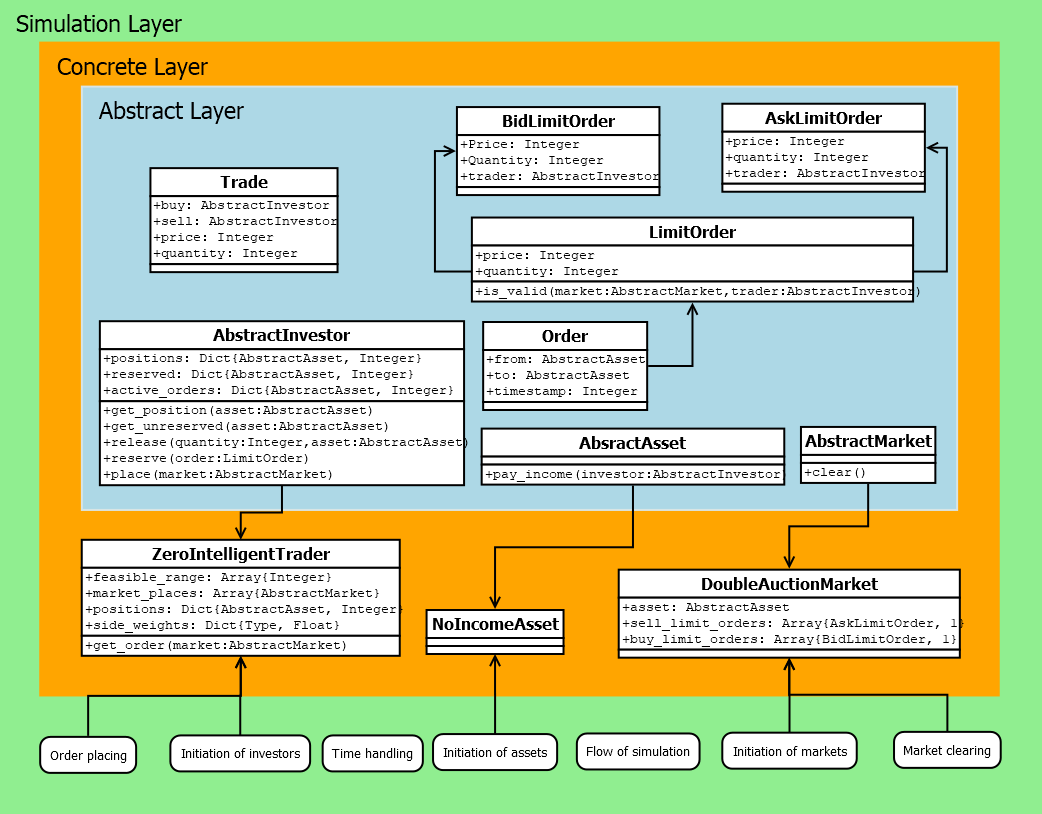
\includegraphics[width=\linewidth]{diagrams/asm_layers.png}
    \caption{Structure of the model}
    \label{fig:asm_structure}
\end{figure}


\subsection{Simulation Process}
% Describe how it works, how the dynamics flow etc.
In a functional sense, the model consists of three main components:
the main level code, traders and markets. The main level code 
orchestrates the flow of the simulation while the components of traders 
and markets handle the pieces of functionalities associated with them. The process
is generalized in ~\ref{fig:sim_proc}. The beginning and the end of the 
simulation are shown in dark orange in the figure. Yellow boxes represent
the actions that belong to the concrete layers and all the actions that
are in the \textit{main} are part of the simulation layer. The remaining belongs
generally to the abstract layer.


\begin{figure}[H]
    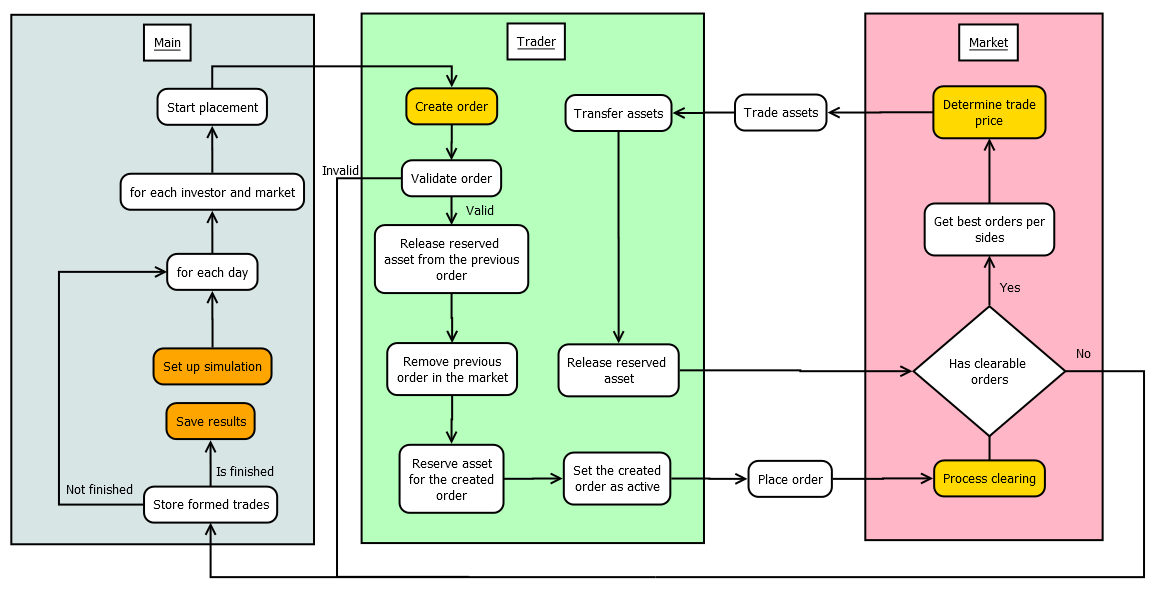
\includegraphics[width=\linewidth]{diagrams/placement_clearing_process.png}
    \caption{Simulation process}
    \label{fig:sim_proc}
\end{figure}

The simulation begins with setting up the parameters such as the number of
trading days and initializing the traders, their assets and the markets.
Then each trading session is iterated over and each trader can create  
an order to each market. After the order creation, the order is validated: 
orders that conflict with the budget constrain are discarded.
The traders have also an option not to create an order. If the order was
valid, the previous order that the trader has made to the same market is cancelled 
and the amount of asset required to execute the order is reserved. The asset
reservation is to prevent the traders from going over with their budgets if they
have allocated the same asset in other markets. Next, the order is
placed to the market and the clearing process begins if the market is a 
continuous double auction. If there are any clearable orders in the clearing process,
they are traded with a price defined by the market type. When
all clearable orders are cleared, the code execution returns to the
main block and either the next trading session is started or the next
trader gets a chance to make orders. In this section, the process of how the
zero-intelligent traders conduct their decisions and how the 
market price formation and clearing works are discussed with more detail.
There are some interesting characteristics in the asset dynamics of this
artificial market and these are also discussed.

\subsubsection{Trader Behaviour}
% How the investors make decisions actually

As mentioned, the traders of the ASM model are zero-intelligent
traders. The reason for this is to minimize the degrees of freedom introduced with 
the model and provide as generic structure as possible. The purpose of the thesis is to 
create an abstract model thus the focus is on microstructure and not in traders' intelligence. The traders' rationality 
for making decisions is reduced to minimum effectively making them unable to speculate, 
manage risks or optimize portfolios. They do not possess the ability to seek profit, 
observe the markets or learn from their previous actions or peers and
they are only able to submit random orders. The mechanics of zero-intelligent traders
are implemented in a way that they are given sets of allowed ranges 
and options in which they choose values randomly. This way the zero-intelligent behaviour is maintained
in addition to have similar options that there are present in real markets 
concerning order placement such as the order quantity, order price and whether
to submit an ask order, a bid order or do nothing. The traders are also budget-constrained
to achieve allocative efficiency as proposed by
\citet{God93}. Budget constrain prevents short selling or borrowing any asset meaning that 
any position cannot end up to be negative.


An order placement decision in the model requires three components 
to be defined by a trader: order side, order quantity and order price. 
There are two possible sides of an order: bid and ask, but
not submitting an order is also a choice. Therefore, the traders
have three options: submitting bid limit order, submitting ask limit order
and not submitting an order. Submitting an order also cancels any previous
order created by the trader to the same market but not submitting an order does not
cancel any previous orders. The traders pick one of these options randomly 
based on the weights specified in the parameters of the simulation run. 

Determining the order price and the order quantity is not completely straight
forward as their feasible ranges cannot be determined completely independently
from each other and the calculations of these ranges differ between bids and asks. Bid order's
value cannot exceed the amount of currency the trader possesses thus this is 
a limiting factor for both, order quantity and order price of a bid. In addition,
the maximum order quantity is inversely proportional to the order price and
therefore if the order price is set first, the maximum order quantity the trader
can set for a bid equals to its amount of currency divided by the price and vice versa. 
However, ask orders do not have such restrictions: the value of an ask order
may not reflect the amount of assets the trader allocates to sell with the order. The
price of an ask order can, in theory, be infinite and the selling trader has no issues
fulfilling the trade on its behalf even though in practice there are no buyers
able to match with such an order. The only limit for the trader placing an ask is the 
amount of the traded asset it possesses: the trader cannot sell more of the asset 
than it has. To summarize, an ask order's feasible ranges for quantity and price 
can be determined independently but this is not the case for bid orders. These feasible 
ranges are shown in ~\ref{eq:feasible_ranges}.

\begin{equation}
\begin{aligned}
% Bid
p_{bid} &= \left[1, pos_{ccy} / q \right] \\
p_{ask} &= \left[1, \infty \right] \\
q_{bid} &= \left[1, pos_{ccy} / p\right] \\
q_{ask} &= \left[1, pos_{asset}\right] \\
\end{aligned}
\label{eq:feasible_ranges}
\end{equation}

To overcome this and to maintain symmetricity between the placement of bids and asks, 
the traders decide the amount of an asset to allocate with an order instead of deciding 
the order quantity directly. This decision is independent on the order price for both
sides and can be handled the same way for both cases. Therefore, a trader placing a bid order 
needs to define the amount of currency to allocate with the trade and a trader placing an ask
order needs to define the amount of the traded asset to allocate, the order quantity in this case. 
The order quantity for a bid is calculated after the amount of asset to allocate 
and the order price have been set. The amount of asset to allocate is drawn from a uniform
distribution in which the minimum is one and the maximum is the amount of the asset the trader
has and is free for allocation. The order price is drawn from a normal distribution in which 
the mean is the last market price. The standard deviation of the distribution is set to a 
constant and the distribution is truncated between one and infinity.

% TODO: Show and discuss about the ranges of the orders

An example of the distribution of order prices and quantities
is shown in ~\ref{fig:generated_orders}. The figure contains a simulation 
of 1 000 000 orders created by a zero-intelligent trader. 
The last market price was set to 1 000 units and the standard deviation of the price to 10. 
The trader possessed 10 000 000 units of currency and 100 000 
units of stock.

\begin{figure}[H]
    \centering
    \begin{subfigure}{.5\textwidth}
      \centering
      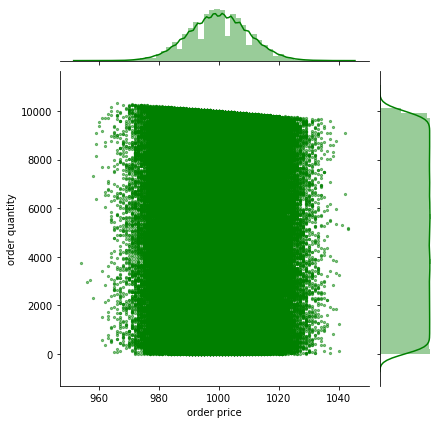
\includegraphics[width=\linewidth]{plots/order_distr_bid.png}
      \caption{Distribution of random bids}
      \label{fig:gener_bids}
    \end{subfigure}%
    \begin{subfigure}{.5\textwidth}
      \centering
      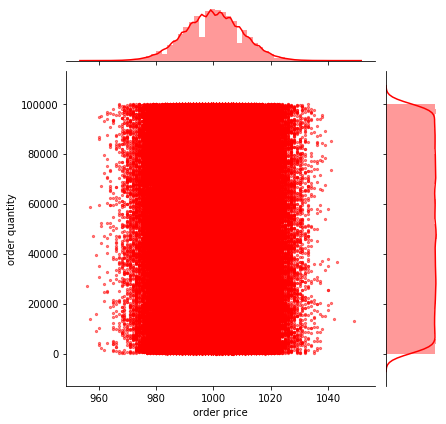
\includegraphics[width=\linewidth]{plots/order_distr_ask.png}
      \caption{Distribution of random asks}
      \label{fig:gener_asks}
    \end{subfigure}
    \caption{Distribution of 1 000 000 random orders}
    \label{fig:generated_orders}
\end{figure}



In the literature, zero-intelligent traders are often implemented differently. For example, in the studies conducted by 
\citet{God93}, \citet{Jam96} and \citet{Mil08} the traders were initially divided into buyers and 
sellers. The traders could trade only one quantity of a stock per order and the order prices 
were drawn from a uniform distribution. However, these markets did not aim for 
realistic market microstructure. The trader behaviour in this model is closer with the Genoa Market 
created by \citet{Genoa01} as in this model the prices are also drawn from a normal distribution and 
the order quantities are derived from the required amount of asset. However, in Genoa Market the 
normal distribution's mean is 10\% higher for ask orders and 10\% lower for bid orders from the 
latest market price in order to increase liquidity. For maintaining simplicity, the mean of the distribution 
is instead set to the last market price in the model of this thesis. Also, the option to not make an order 
seems not to be prevalent in the previous literature. However, \citet{Raberto05} implemented waiting times and order 
cancellation after specified times which may produce similar behaviour. 

\subsubsection{Time Handling}

The implementation of time in the simulation took inspiration from the asynchronous model created by \citet{Julien07}. 
As in their ASM model, in this model the traders are randomly given the ability to speak and make 
their trading decisions. The proportion of traders allowed to make a decision is defined in
\textit{speak ratio} which is a parameter for the simulation. After randomly selecting the traders
according to the speak ratio, this set of traders is shuffled randomly and are asked to do trading 
decisions one by one for each market. However, it is unclear how the interval between placement 
decisions should be interpreted in terms of real-time units such as seconds or minutes. In addition, 
the issue of nontrading is also inherently present in the model: the time interval between trades 
is non-fixed.

The submitted orders and created trades also include timestamps. For orders, the timestamps are used
to determine the comparable age of each order. This is useful for clearing mechanics that sort 
order by their age to determine the clearing price. In the case of trades, this information
is useful for analytical purposes to determine the timeline of events. A timestamp is simply 
an integer starting from one at the beginning of the simulation and has no additional 
intended representation. Each checking of time increments the global time with one unit.

\subsubsection{Market Mechanics}
% How the market is cleared actually 

The market is a continuous and double auction in nature.
The clearing mechanics themselves are, however, 
rather the same as could be for a call market: 
the orders are cleared until there
are no bid orders with price equal or exceeding the
ask order with the lowest price. 
Continuity is achieved by launching the clearing process
every time an order arrives at the market. 
The clearing mechanics are defined in 
the abstraction layer in a way that the same body
of code works for call markets and continuous markets
and the distinction between the markets, such as how 
the market price is formed, is handled inside the clearing
mechanics by calling the parametrized functions that are 
defined explicitly for each concrete market type. 
The main body of the clearing function, 
as written in the source code, is shown in the listing ~\ref{lst:clearing}.
In the listing, the clearing price resembles the market price
of the clearing session which is calculated for call markets but not for 
continuous markets. For continuous markets this price is simply nothing and
the price determined from a pair of crossing orders is used instead using function
\emph{get\_trade\_price}. The rationale for the complexity is that in future experiments
that study call markets could utilize the same code without modifications 
even though call markets are not studied in this thesis.

It should be noted that this mechanic may not be optimal in terms of performance: 
only the newly submitted order may possibly be cleared and therefore a more 
optimized solution could utilize the fact that only this order and the opposing book 
need to be compared and not necessarily both books themselves. However, 
in this case simplicity was considered more important than the speed of the code execution.


\begin{lstlisting}[caption={Clearing process},label={lst:clearing}]
...
# The clearing price is defined here
# in case of call market. Nothing
# should be returned if the price
# is defined per order pair basis
clearing_price = get_trade_price(market)
while maxprice(buy_book) >= minprice(sell_book)

    order_sell = get_best(sell_book)
    order_buy = get_best(buy_book)
    
    # trade_price is clearing_price if defined,
    # else calculated per order pairs
    trade_price = (
        ~isnothing(clearing_price) ? 
        clearing_price
        : get_trade_price(order_buy, order_sell, market=market)
    )

    trade = trade!(
        order_buy, order_sell, 
        price=trade_price, 
        from=market.currency, 
        to=market.traded_asset
    )
    ...
\end{lstlisting}

The price formation of the continuous market is implemented
on the order pair basis. The trade price is simply the price
stated in the older order of the paired orders. % SOURCE: find a source to describe why this way the price
The quantity of the trade is chosen from the smaller of the two orders
and the bigger order is partially cleared in case they were not 
equally sized.

% About literature


\subsubsection{Handling of Assets}
% Why use integers as units for assets

The model is constructed in a way that enables usage of multiple assets
and the assets are handled symmetrically. The former is achieved with
allowing multi-asset positions and multi-asset reservation and 
it is the simulation layer's responsibility to create the assets and the 
markets for them and ask the investors to create orders in these markets. 

Asset symmetricity means that there is no universal or central currency 
and the currencies are handled as any other asset. In a theoretical sense, 
currencies are also just investment options and there is no inherent reason why other 
asset classes, such as stocks, could not operate as the definition 
of value. This feature creates complexity to the model compared to a model
with a central currency acting as the baseline for value but it also enables an
abstracted structure that handles natively cross-currency
markets or ecosystems in which there exist markets between assets A and 
B and between B and C but not between A and C. This is also a better 
representation of theoretical markets.

Support for multiple assets and asset symmetricity is constructed by storing 
the owned and reserved assets of a trader to the same data structures regardless
of the type of asset in question. Each trader has one dictionary for positions 
and one for reserved assets and the keys for the dictionaries are the assets. 
In addition, the markets also contain information about the assets traded with and traded to 
in the market. Each market has an attribute, or a field as called
in Julia, for the asset traded with in the market and for the asset
traded to in the market. As order submission occurs on a market basis, this information
is used to determine what asset should be allocated from the trader's reserve as a result of 
order submission and to determine the assets to exchange when a trade is formed in a market. 
The orders need not have the information about the assets in question as all orders are always
market-specific in the model and never passed around without the context of which market they are 
for. This mechanic also allows interesting ecosystems such as environments
in which multiple identical markets can coexist that trade the same asset using the same asset as
currency. 

% Asset allocation, reserve & active orders
% TODO: UPDATE: wording is less shit but still shit
In single market models, disallowing the orders that would require more assets to execute
than there is in the trader's position should be sufficient to maintain the budget constrain. 
However, for a multi-market ecosystem this is not enough. The quantities of an asset 
that are already allocated to a market via orders must be kept track of and the total amounts of 
allocated quantities must not exceed the actual asset positions of the trader. If the maximum allowed 
allocation is not enforced and if one trader has submitted multiple orders trading the same asset
there is a chance that the trader's asset or currency position goes negative. 
To prevent this, in this ASM model all of the allocated assets, called reserved asset 
in the simulation, are kept track of in addition to the actual asset positions. The model also
accepts only one order per trader per market as it makes little sense that
the traders are allowed to express multiple different opinions to one market 
simultaneously: especially having a bid and an ask orders on the same market
at the same time may lead to a confusing pattern where a trader is trading with
itself and therefore artificially pumping up the liquidity of the market. 

In addition to these, the latest and unfulfilled order that a trader has already placed
to a market is tracked in the trader's data structure to make cancellation easy
but also to implement a relevant additional feature: active order lookup. To prevent that
the placing of a new order is not limited to the trader's existing order in the market,
the effect of this previous order, called active order, in the asset reverse is excluded. 
This active order will be cancelled as soon as the new order is validated and the new order
will immediately become the active order. By doing so, the traders' placement is less 
conservative without breaching the budget constrains.


% Integers & bid-ask asymmetricity
All quantities of the assets are stored as integers to prevent wealth leakage 
or creation because of the floating-point arithmetics. Using integers also
conveniently act as the tick size for all the markets. This also has the side effect
of that all the prices must be represented as integers as one piece
of a traded asset must equal the exact quantity of the asset used as a currency
in the market. Furthermore, this creates inefficiency in the market if the quantities
of owned assets are small and a phenomenon of asymmetricity between bidders and askers
araises. The price set by a seller can be virtually anything: they can set
arbitrary positive price for their order as the only limitation is the amount
of traded asset they can commit to the order which is independent on the price. 
Every increment in order price means more profit for the seller
if the order is executed. On the other hand, because of the 
lower limit of one in the order price, a buyer does not have the same freedom.
The maximum price a buyer can set equals the quantity of the currency 
the buyer holds but the minimum price is one. This is
illustrated in the figure ~\ref{fig:buy_sell_asym} in which the all possible
combinations of quantities and prices are shown for a buyer who owns ten units 
of currency and for a seller who owns ten units of the traded asset. 
The coloured areas represent where the possible combinations lie. 

 % And what this causes etc.
 % Price can be anything for seller but for buyer, there are boundaries

 \begin{figure}[H]
    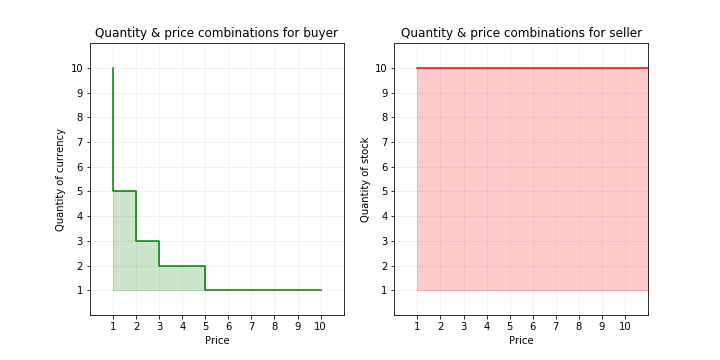
\includegraphics[width=\linewidth]{plots/buyer_seller_asymmetricity.png}
    \caption{Illustration of buyer-seller asymmetricity}
    \label{fig:buy_sell_asym}
\end{figure}

The ASM literature does not address this issue and the discussion about 
tick sizes in ASM models is scarce. The models created in previous studies 
may use floating points and accept the slight, perhaps minimal, spillover 
of assets in the system. \citet{FloatingPoint06} warned about the effects 
floating-point errors may have in the perspective of agent-based models. 
They stated there is no solution that fits all problems but introduced 
several methods to mitigate the problem such as interval arithmetics. They, 
however, did not discuss the tick sizes.

The bid-ask asymmetricity may become an issue when the price of the market
approaches to one. Near the price of one the tick size begins to reduce the efficiency
of the markets: for example, if the market price is four units the minimum movement 
of the price is 25\% up or down. In addition, there may be an issue that the efficient
price cannot be reached if it lies under the price of one. Probably
the simplest solution to avoid this while still having integers for quantities 
of assets is to make sure the traded asset has sufficiently high value
compared to the currency of the market. This can be achieved simply injecting
enough currency to the ecosystem to inflate the price. Another interesting 
solution to mitigate the problem of potentially unreachable efficient price 
is to have two markets for the same asset pairs but opposing direction. 
The first market trades an asset \textit{A} with an asset \textit{B} but the 
other market trades the asset \textit{B} with the asset \textit{A}. 
The price of the other market should, in theory, be the multiplicative inverse of 
the market price in the opposing market. This solution is simulated in the figure 
~\ref{fig:opposing_markets}. The total amount of stock is increasing, 
thus inflating, and the total amount of currency is decreasing, thus deflating, 
with constant rates in the example. When the equilibrium price for the stock 
decreases to below one the trading begins in the opposing market. 



\begin{figure}[H]
    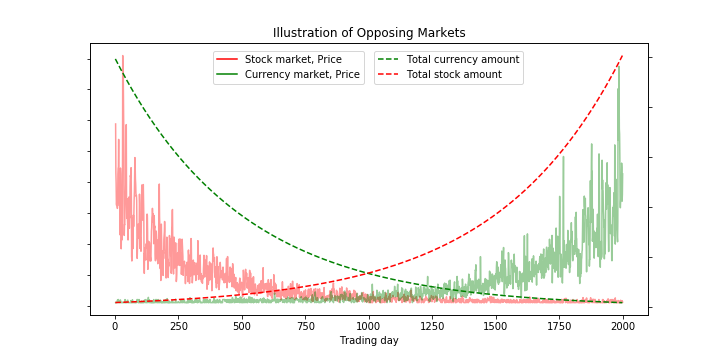
\includegraphics[width=\linewidth]{plots/opposing_markets.png}
    \caption{Two markets with inverse assets}
    \label{fig:opposing_markets}
\end{figure}



In the simulations conducted in this thesis, the simpler approach was chosen. 
The global quantities of assets are set high enough so that it is improbable 
for the market price to decrease too low. 
% implmenentation of payoffs (dividend, interests etc)

% How the literature
%Most of the ASM literature study only ecosystems in which
%the traders can only trade a stock with a cash.